\chapter{Introduction}
\label{chap:introduction}
\section{Motivation and Background}
Mission operations are one of the most critical aspects of any space mission.
They involve the planning, execution, and monitoring of all activities to ensure science goals are met and the safety of the instrument is maintained.
With more complex instruments and larger data volumes, mission operations have become increasingly challenging.
Missions such as Mars Science Laboratory (MSL), Roman Space Telescope (RST), and the Astrophysics Stratospheric Telescope for High Spectral Resolution Observations at Submillimeter-wavelengths (ASHTORS) have a demonstrated need to quickly analyze data in order to meet the ever shrinking operation timelines of modern space missions \parencite{wilson2017nasa}.
This demand for rapid tactical decision-making in bandwidth constrained environments has led to the need for more efficient ways to review and analyze data.

Traditional data analysis approaches often rely on manual inspection or, in the case of bandwidth limited systems, random sampling of data to identify potential issues or spot novel features.
When looking for unexpected and uncharacterized phenomena, these approaches can be inefficient and time-consuming as it is easy to overlook important features without a systematic approach.
Novelty detection is particularly well suited for this task as it does not rely on a priori knowledge of what constitutes an anomaly, simply that there is a set of data that is representative of the expected behavior of the system that can be used to measure how well new data matches this expected behavior \parencite{japkowicz1995novelty}.
This need for rapid anomaly detection has led to the development of new methods and techniques that can quickly identify unexpected features in data, allowing for more efficient mission operations \parencite{kerner2020comparison}.
While much of the work in this area is focused on the development of new algorithms and techniques, there is also a need for more efficient ways to implement these methods in practice.
This is where the use of modern software engineering practices and tools can play a critical role.

\section{Research Objectives}
The primary goal of this dissertation is to develop a framework for data prioritization that allows mission operations teams to quickly triage targets for analysis and review.
Novelty detection is a key component of this framework, as it allows for the identification of unexpected features without prior knowledge of what constitutes an anomaly.
This gives it the versatility to be applied to a wide range of data types and mission scenarios.
For our domains of interest, I focused on the use of novelty detection to identify features in multispectral images from Mastcam on MSL \cite{horton2021integrating}, snowballs and cosmic rays on RST's Wide Field Instrument (WFI) \cite{horton2024anomaly}, and finally anomalous spectra on ASTHROS \cite{horton2024board}.
In addition to scientifically different domains, these three instruments differ in their operational domains, with MSL being a currently operational mission analyzing data while in the field, RST being a future mission using data collected during integration and testing to identify potential issues, and ASTHROS also being a future mission but with the goal of performing this analysis onboard the instrument.

\begin{figure}
\centering
\includegraphics[width=0.8\textwidth]{figs/intro/asthros.png}
\caption[The Astrophysics Stratospheric Telescope for High Spectral Resolution Observations at Submillimeter-wavelengths (ASTHROS)]{
    ASTHROS in the high bay of the Columbia Scientific Balloon Facility (CSBF) in Palestine, Texas. 
    The gold and black structure is the telescope and readout system, while the white structure is the gondola that will carry the instrument into the stratosphere. 
}
\label{intro/fig:asthros}
\end{figure}

ASTHROS, shown in Figure \ref{intro/fig:asthros}, is a major component of this dissertation as it was at a scale that allowed us to develop a complete end-to-end system with the implementation of onboard novelty detection in mind. 
ASTHROS is a scientific ballooning mission that gives us the opportunity to perform high spectral resolution observations at submillimeter wavelengths from the stratosphere \parencite{siles2020asthros}.
Ballooning literally gives astronomers a much higher vantage point to observe than ground based telescopes by allowing us to get above the majority of the atmosphere, which is a major source of noise in submillimeter observations \cite{yajima2009scientific}.
Figure \ref{intro/fig:atmosphere} shows the atmospheric opacity at various wavelengths, with the submillimeter wavelengths (100-1000 $\mu$m) being completely opaque from the ground.

\begin{figure}
\centering
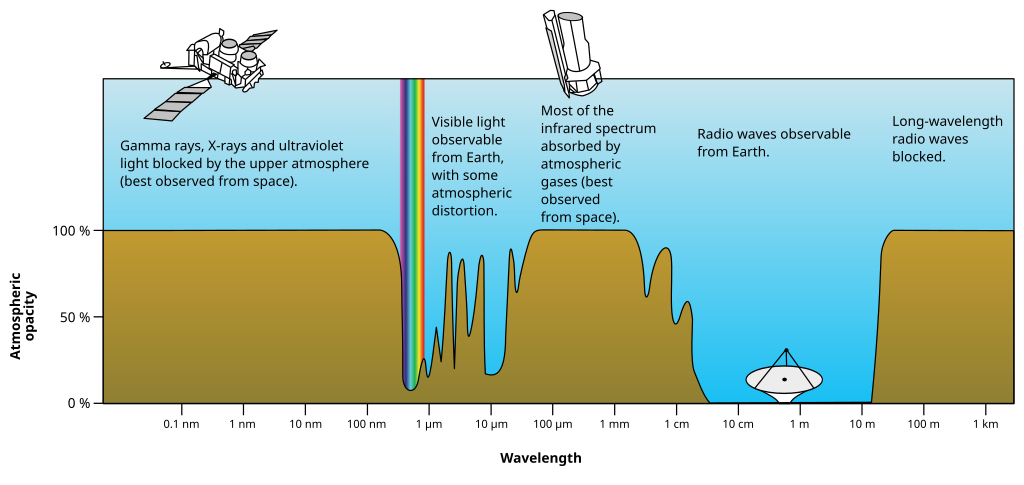
\includegraphics[width=0.8\textwidth]{figs/intro/atmosphere.png}
\caption[Atmospheric Opacity at Various Wavelengths]{
    The atmospheric opacity at various wavelengths, showing the submillimeter wavelengths (100-1000 $\mu$m) being completely opaque from the ground.
    This makes ballooning a critical component of submillimeter astronomy. NASA (original); SVG by Mysid., Public domain, via Wikimedia Commons.
    \label{intro/fig:atmosphere}
}
\end{figure}

This higher vantage point is not without its drawbacks, however, as communication with the instrument has limited bandwidth and latency. 
Because of this, ballooning mission store all of their data on board the instrument and only send back samples of the data for diagnostic purposes.
When the balloon lands, the instrument is recovered and the hard drives are read to review the full dataset \parencite{walker_STO}.
This makes it an ideal candidate for on board novelty detection, as I can use the limited bandwidth to send only the most diagnostically relevant data back to the ground for review.
In our case, this is data that differs from the expected behavior of the instrument, which is what novelty detection is designed to identify.

\begin{figure}
\centering
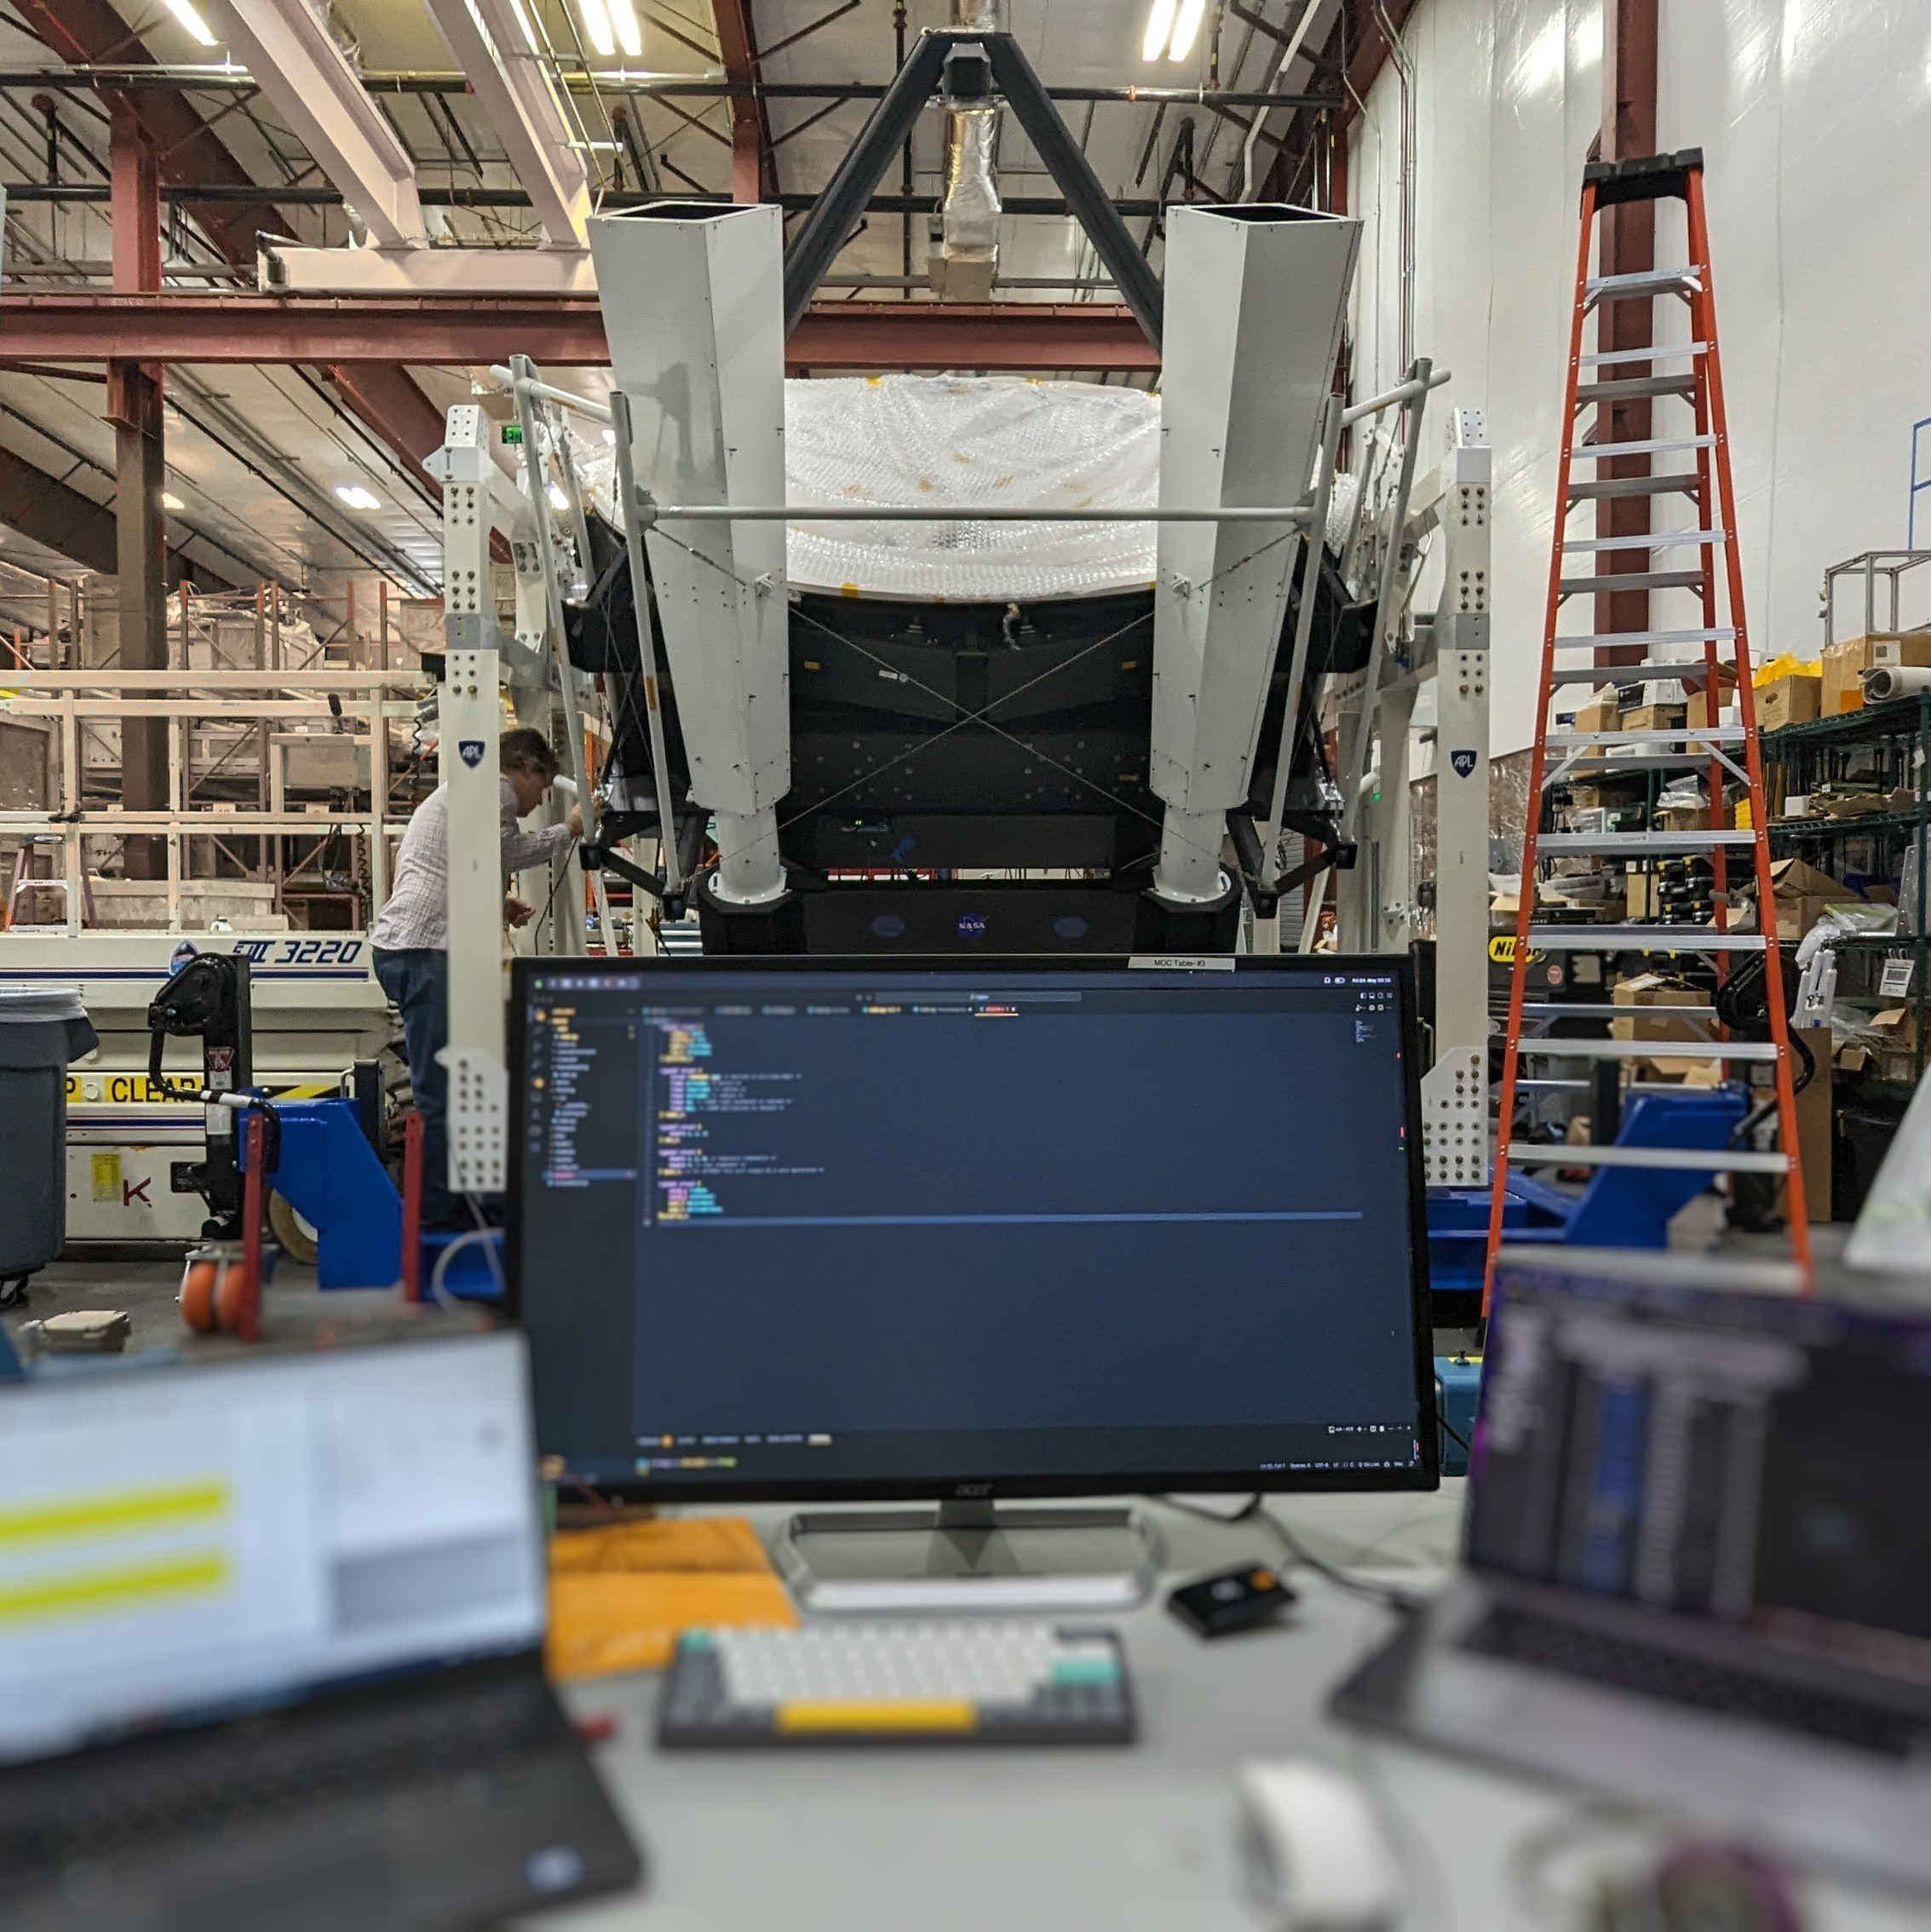
\includegraphics[width=0.8\textwidth]{figs/intro/asthros_instrument.jpg}
\caption[Command Station for Software Development of ASTHROS]{
    My vantage point for developing ASTHROS, sitting in front of the instrument to test systems and software.
}`'
\label{intro/fig:asthros_instrument}
\end{figure}

ASTHROS, being in its early stages of development, also made it an ideal candidate for me as a graduate student to develop a complete end-to-end system.
This allowed me to work closely with the instrument team to develop a system that meets their needs and can be integrated into the instrument's operations.
Developing this system allowed me to utilize all aspects of my background, from my Software Engineering and Applied Physics degrees to my growth as a scientist and engineer during my Ph.D program.
Figure \ref{intro/fig:asthros_instrument} shows my own vantage point in developing this instrument, as I sat front and center controlling every aspect of the instrument's software. 
I played a critical role in the development of the instrument's software, from the low-level hardware control to the high-level data analysis and visualization tools.
My objective in all this was to develop a system that functionally met the science goals of the mission while also giving me a platform to integrate novelty detection into the instrument's operations during flight. '

\section{Chapter Overview}
This dissertation is organized into several chapters, each focusing on a different aspect of the research and development process.
Throughout my time as a graduate student, I had many published works that contributed to this dissertation, and I have included them in the relevant chapters in their entirety with modifications to fit the overall narrative of the dissertation or add additional work done since their publication for the sake of completeness.
Any changes to these works are noted in the prelude to each chapter.

Chapter \ref{ch:msl}, Data Discovery Systems for Planetary Science,  was my first published work from \cite{horton2021integrating}, where I developed a system to integrate novelty detection into the operations of MSL.
This work has a strong focus on background knowledge about novelty detection, as well as the development of a system to integrate novelty detection into the operations of MSL.
This being one of the first projects I worked on, laid the foundation for my future work as I began to adapt the system for other instruments and missions.

Chapter \ref{ch:rst}, Anomaly Detection for the Roman Space Telescope Wide Field Instrument's Science Data Processing Pipeline, builds on the work done in Chapter \ref{ch:msl} and focuses on the development of a system to integrate novelty detection into the integration and testing (I\&T) of RST WFI.
With the support of a NASA Space Technology Graduate Research Opportunity (NSTGRO) fellowship, I began working with the RST WFI I\&T Science Data Pipeline team to develop a system that could identify snowballs and cosmic rays in their data. 
This work culminated in the publication of \cite{horton2024anomaly}, which describes our approach to identifying these anomalies. 

Following that, Chapter \ref{ch:spectra}, On-Board Science Data Quality Analysis using Anomaly Detection for ASTHROS, focuses on the development of a system to integrate novelty detection into the operations of ASTHROS.
This chapter is the first of three that focuses on my work with ASTHROS, the primary instrument for this dissertation.
Chapter \ref{ch:spectra} is based on the publication \cite{horton2024board}, which describe our on-board approach to identifying anomalous spectra in the data collected by ASTHROS.
This is done by adapting the multispectral system developed in Chapter \ref{ch:msl} to work with the raw spectra collected by ASTHROS.

Chapter \ref{ch:carina}, Electron Density Mapping in the Carina Nebula, is a departure from the previous chapters on novelty detection and focuses on one of the science goals of ASTHROS, mapping Carina Nebula. 
ASTHROS will be utilizing the ratio of [NII] 122 $\mu$m and 205 $\mu$m lines to map the electron density in the Carina Nebula.
This chapter explores new [NII] 205 $\mu$m data from the Stratospheric Observatory for Infrared Astronomy (SOFIA) to create a map of electron density with Radio Recombination Line (RRL) data from the Deep Space Network (DSN) and Radio Continuum maps from the Atacama Large Millimeter/submillimeter Array (ALMA).
While this might seem unrelated to the overall goals of this dissertation, a critical component for developing systems is understanding the users and their needs.
By becoming a member of the ASTHROS science team and having a vested interest in the science goals of the mission, I am able to better understand the mission's needs and develop a system that targets the pain points of the scientists.
While this work has not yet been published, I have plans to add more analysis to the data and submit it to The Astrophysical Journal in the near future.

Finally, Chapter \ref{ch:readout}, ASTHROS Payload Readout System Design, focuses on the development of the payload readout system for ASTHROS.
This chapter is essentially a user manual for every aspect of the readout system, from the low-level hardware drivers to the high-level interfaces used to control the entire payload.
The manual outlines the design choices made during the development of the system and why they were made in service of both the science goals of the mission as well as additions made to support integrating novelty detection into the mission operations of ASTHROS.
For the sake of completeness, this chapter is long and detailed, as it is intended to be a standalone document that can be used by the ASTHROS team to understand how each system works and how to use it.

We end with our conclusions and future work in Chapter \ref{ch:conclusion}.
This chapter summarizes the key findings of the dissertation and discusses to what extent we've covered the title, "Development, Implementation, and Impacts of Novelty Detection Systems for Mission Operations."
We evaluate what each of those three components in the title means and how they relate to the work done in this dissertation.
And finally, we discuss the future work that can be done to measure the impacts of these systems during a flight, and improve the scientific software development process as a whole.